\documentclass{llncs}
\pagestyle{headings}   % turn on page numbers
\usepackage{epsf}
\usepackage{epsfig}

\usepackage{url}

\newcommand{\Circus}{{\sf\slshape Circus}}
\newcommand{\Class}[1]{\texttt{#1}}
\newcommand{\Element}[1]{\texttt{#1}}
\newcommand{\Interface}[1]{\texttt{#1}}
\newcommand{\Method}[1]{\texttt{#1}}

\begin{document}
\title{CZT Support for Z Extensions}
\author{Leo Freitas$^1$ \and Tim Miller$^2$ \and Petra Malik$^3$ \and Mark Utting$^3$}

\institute{%
   \begin{tabular}{cc}
      University of York, UK  $\quad\quad$ & University of Liverpool, UK
      \\ %
      $^1$\texttt{leo@cs.york.ac.uk} $\quad\quad$ & $^2$\texttt{tim@csc.liv.ac.uk}
   \end{tabular}
   \begin{tabular}{c}
      University of Waikato, New Zealand
      \\ %
       $^3$\texttt{\{petra, marku\}@cs.waikato.ac.nz}
   \end{tabular}
} %

\maketitle


\begin{abstract}
  The Community Z Tools (CZT) is an integrated
  framework for the Z formal specification language.  In this
  paper, we show how it is also designed to support extensions
  of Z, in a way that minimises the work required to build a
  new Z extension.  The goals of the framework are to maximise
  extensibility and reuse, and minimise code duplication and
  maintenance effort.  To achieve these goals, CZT uses a variety of
  different reuse mechanisms, including generation of Java
  code from a hierarchy of XML schemas, XML templates for shared
  code, and several design patterns for maximising reuse of Java
  algorithms.
  %
  The CZT framework is being used to implement several integrated
  formal methods, which add object-orientation, real-time features
  and process algebra extensions to Z.  The effort required to
  implement such extensions of Z has been dramatically reduced
  by using the CZT framework.

  \noindent
  \textbf{Keywords}: Standard Z, Object-Z, \Circus, TCOZ, design patterns,
     framework, AST, parsing, typechecking, animation.
\end{abstract}

\section{Introduction} \label{sec:intro}

  The Z language~\cite{isoz} is a formal specification notation that
  can be used to precisely specify the behaviour of systems, and
  analyse it via proof, animation, test generation, and so on.
  Z was approved as an ISO standard in 2002, but currently there are few
  tools that conform to the standard.\footnote{CADiZ
  (\url{http://www-users.cs.york.ac.uk/~ian/cadiz}) is the only Z tool
  that conforms closely to the Z standard.  It is freely available,
  but is not open source and does not aim at supporting Z extensions.}
  The Community Z Tools (CZT) project~\cite{czt} is an open-source Java
  framework for building formal methods tools for standard Z and Z extensions.

  CZT provides the basic tools expected in a Z environment, such as
  conversion between \LaTeX, Unicode and XML formats for Z, and
  parsing, unparsing, typechecking and animation tools, with a WYSIWYG
  Z editing environment integrated within the
  jEdit\footnote{See \url{http://www.jedit.org}.} editor.
  There are also several more experimental tools under development,
  such as a Z-to-B translator and a semi-automated GUI-builder for
  Z specifications.  However, the main design goal of CZT is to
  provide a framework which makes it easy to develop new Z tools.
  This paper describes how the framework also makes it easy to develop
  tools for extensions of Z.

  In recent years, there has been an increasing interest in combining
  different programming paradigms within an uniform formal notation,
  where Z plays a central role. This has given rise to many Z
  extensions, which add features such as
  %
  process algebras~\cite{fischer-1998,fischer-2000,circus.sem:intro},
  object orientation~\cite{oz,ohcircus},
  time~\cite{tcoz,circus.sem:real.time2},
  mobility~\cite{circus.sem:mobility}, and so forth.

  Among these extensions, CZT supports Object-Z~\cite{oz}, a
  specification language that extends Z with modularity and reuse
  constructs that resemble the object-oriented programming
  paradigm. Such constructs include classes, inheritance, and
  polymorphism. CZT supports Object-Z in the form of parsing,
  typechecking, and other facilities.  Currently, we are working on
  extensions for Timed Communicating Object-Z (TCOZ)~\cite{tcoz},
  which is a blend of Object-Z and Timed-CSP~\cite{timed-csp}, as well
  as extensions for \Circus~\cite{circus.sem:intro}, a unified
  refinement language that combines Z, CSP~\cite{csp.books:roscoe},
  and the refinement calculus~\cite{fm.ref:morgan}, with Hoare and
  He's \textit{Unifying Theories of Programming} (UTP) as the semantic
  background~\cite{hoare.utp}.

  This paper describes the engineering techniques used in the CZT framework
  to maximise extensibility and reuse.
  Most of these techniques could also be applied to frameworks
  for other integrated formal methods, especially when the
  framework must support several different extensions of a common
  base language (like the role of Z in CZT).

  In Section~\ref{xml-schemas}, we present a method for specifying an
  XML interchange format that maximises extensibility.
  Section~\ref{java-ast-classes} describes the automatic generation
  and design of the \emph{Annotated Syntax Tree} (AST) classes.
  Section~\ref{parsers} presents a method for generating parsers,
  scanners, and other related tools for the different Z extensions,
  and Section~\ref{typecheckers} presents the design of the CZT
  typecheckers, which are tailored for extendibility and
  reuse. Section~\ref{animation} presents the animation method used in
  the CZT animator, ZLive, and discusses the possibility of using this
  to animate extensions to Z. Section~\ref{section-manager} presents
  the design of the {\em specification manager}, an integral component
  of CZT that caches information about specifications to improve the
  efficiency of the tools.  Section~\ref{sec:conclusions} concludes
  the paper and discusses the future of the CZT project.


\section{XML Schemas}
\label{xml-schemas}

  The first step in designing the CZT tools and libraries was the
  development of an XML schema that describes an XML markup for Z
  specifications (ZML)~\cite{UttEA:03}.  This is an interchange format
  that can be used to exchange parsed Z specifications between
  sessions and tools.

  Standard Z allows specifications to be exchanged using Unicode,
  \LaTeX\ or e-mail markup.  However, implementing a parser for such
  specifications is a non-trivial task that can take several months.
  ZML, in contrast, can be parsed
  immediately using one of the available XML parsers like
  Xerces\footnote{See~\url{http://xml.apache.org/xerces-j/}} or
  Crimson\footnote{See~\url{http://xml.apache.org/crimson/}}.
  An important advantage of XML is that it allows
  exchange between tools written in different languages, since virtually
  all programming languages provide XML reading and writing libraries.

  The idea of using Z with XML has also been explored in the
  Z/Eves theorem prover~\cite{tp.tools:zeves.ref}.  It allows one to
  create a customised theorem prover with additional tactics tailored
  for a particular specification by modifying the XML representation
  of the Z specification in Z/Eves~\cite{tp.tools:zeves.api}.
  The main problem however, was the lack of a common standard.

  The XML schema for ZML was carefully designed, via consensus between
  several groups of interested people, by selecting the best features
  of the abstract syntaxes of CADiZ, Zeta and the Z standard.
  ZML supports several kinds of extensibility:
  \begin{description}
  \item[Extensible Annotations:] Each Z construct can be \emph{annotated}
    with arbitrary information, such as type information, comments,
    anticipated usage, source-file location.
  \item[Extensible Expressions, Predicates, Paragraphs etc:] This
    allows Z extensions to add new kinds of expressions, paragraphs etc.
  \item[Extensible Schemas:] The standard XML schema features, such as
    namespaces and importing, mean that Z extensions can be defined without
    modifying the original ZML schema.
  \end{description}
  The following strategies have been used to achieve these kinds
  of extensibility.

  The \textit{``any''} element can be used in an XML schema to enable
  instance XML documents to contain additional elements not specified
  by the schema.  This concept has been used to define annotations.
  That is, an annotation to a term can either be one of the
  annotations defined in the XML schema for Z, or any other kind of
  data.  New kinds of annotations can be added without changing the ZML
  schema.  This allows a tool builder to decide what data makes sense
  for a particular tool.  Tools that do not use a particular kind
  of annotation simply ignore those annotations.

  A typical style of defining XML schemas or DTDs is to explicitly
  list the possible alternatives for expressions, predicates, \textit{etc}.
  This makes it difficult to extend the syntax of expressions or
  predicates.  In contrast, ZML uses \emph{inheritance}
  (\emph{substitution groups} in XML schema terminology) extensively
  throughout the XML schema.  Abstract elements are used to provide
  placeholders for their derived elements.  For example, the abstract
  element \Element{Para} is the parent of all concrete Z paragraphs,
  such as axiomatic paragraphs (element \Element{AxPara}), and free
  types paragraph (element \Element{FreePara}).  Other elements that
  contain paragraphs, like Z section (element \Element{ZSect}), are
  defined to contain a \emph{reference} to the abstract \Element{Para}
  element.  This allows any subtype of \Element{Para} to be used
  instead.  This has the same extensibility advantages as subtyping
  in object-oriented languages.

  A Z extension can add new kinds of paragraphs, expressions and predicates
  etc.~simply by extending these ZML inheritance hierarchies.  It is
  important to note that this can be done without modifying the
  ZML schema file.  Instead, the Z extension creates a new XML schema
  which \emph{imports} the original ZML schema file, then defines the
  additional constructs using a new namespace.
  This means that several separate extensions of Z can easily coexist.
  For example, the XML schema for Object-Z imports
  the ZML schema file, and defines a new paragraph for classes (element
  \Element{ClassPara}) that is derived from element \Element{Para}
  defined in the ZML schema.  Instance documents of the Object-Z
  schema can now contain class paragraphs in addition to the standard Z
  paragraphs wherever an element \Element{Para} is expected.  Thus,
  an Object-Z specification in XML format can contain a mixture of
  Z and Object-Z constructs, such as:
\begin{small}
\begin{verbatim}
    <Z:ZSect>
      <OZ:ClassPara> ...  <Z:True/> ... </OZ:ClassPara>
    </Z:ZSect>
\end{verbatim}
\end{small}

  This process of extending the XML schema can be done multiple times, so
  that even a Z extension can be extended.  For example, the
  additional elements provided by the Object-Z XML schema are further
  extended by the TCOZ XML schema.  Again, the definitions of the elements
  for TCOZ are encapsulated into a TCOZ XML schema file, and the ZML and
  Object-Z XML schemas do not need to be modified.
  Similarly, the \Circus\ extension for CZT is encapsulated into a
  \Circus\ XML schema file that extends the main standard Z schema.
  This approach of extension via inclusion is explored throughout the
  different layers of CZT tools.
  The resulting net effect is that once one package is finished, it
  can be directly extended through inheritance, hence simplifying the
  task of extending standard Z to a great extent.

  The use of XML in the CZT has proved to be an efficient and extensible
  solution for representing a Z specification and its extensions.  The
  XML approach helps to clarify design decisions in a straightforward
  fashion.  This representation is the key for the integrated
  development and exchange of information among different Z tools.

\section{Java AST Classes}\label{java-ast-classes}

  To manipulate Z \emph{Annotated Syntax Trees} (AST) within Java (or
  any other programming language), we must convert ZML files into Java
  objects.  This could easily be done using one of the Java XML
  reader/writer libraries, such as DOM, but this would result in a
  very generic interface to the Java objects --- to the programmer they
  would appear to be an N-ary tree of \texttt{Element} and
  \texttt{Text} objects. This does not accurately reflect the Z
  syntax or semantics, is not elegant, and is error-prone to use.

  Instead, we provide a customised Java interface for each Z
  construct, with appropriately named \emph{get} and \emph{set}
  methods for each subcomponent.  This makes programs more readable,
  and provides much stronger type checking.  However, there are some
  situations where the generic N-ary tree view is more convenient
  (for example, writing a deep copy procedure), so our Java interfaces
  also provide a low-level generic view of each node, via the following
  two methods:
\begin{small}
\begin{verbatim}
    Object[] getChildren();  // return all children of this node
    Term create(Object[] args); // create a new version of this node,
                                // with the given children.
\end{verbatim}
\end{small}
  Having these two alternative views of each node of the AST gives
  the best of both worlds --- one can write generic tree traversal
  algorithms, as well as readable and type-safe Z-specific syntax
  manipulations.

  In fact, these CZT Java AST interfaces and their implementation
  classes are automatically generated from the XML schemas described
  in the previous section, using our code generator \emph{GnAST}
  (GeNerator for AST).  The generated code looks similar to the code
  Java data binding tools like
  JAXB\footnote{See~\url{http://java.sun.com/xml/jaxb/}} or
  Castor\footnote{See~\url{http://www.castor.org/}} are
  producing. While the main purpose of a Java binding tool is to
  provide the ability to convert from XML format to Java objects and
  vice versa, the main purpose of GnAST is to generate well-designed
  AST classes.  For example, the AST classes generated by GnAST
  support an extensible variant of the visitor design pattern.

  The automatic AST generation from the XML schemas dramatically
  reduces the time required to develop a new Z extension, ensures a
  common style of interface, and improves maintainability.  For
  instance, the complete AST folder representing standard Z contains
  around $420$ Java files.  GnAST has also been used to generate AST
  interfaces and classes for Object-Z, TCOZ, and \Circus.  In total,
  from the four XML schema files for standard Z and its extensions,
  GnAST automatically generates around $2300$ Java files.  This
  provides a very convenient and consistent way to obtain AST interfaces
  and classes for Z extensions that fit well into the AST for standard Z.
  That is, the AST classes for Z extensions also support the visitor design
  pattern described below.

  The visitor design pattern~\cite{GamEA:95,MaiCha:01} makes it very
  easy to write tools like typecheckers and printers, which need to
  traverse an AST.  It allows new traversal operations to be defined
  without modifying the AST classes.  To define a new operation, all
  you need to do is to implement a new visitor class.

  The visitor design pattern used in CZT has been described in detail
  in~\cite{czt}.  It is a variant of of the \emph{acyclic
  visitor}~\cite{Mar:97} pattern and the \emph{default
  visitor}~\cite{Nor:97} pattern.  Its main advantages are that it
  allows the AST interfaces and classes to be extended without
  affecting existing visitors, and that it allows a visitor to take
  advantage of the AST inheritance relationships.
  For example, a copy visitor that copies an AST can
  provide a default behaviour for \Interface{Term}, the base of the
  AST inheritance hierarchy.  Since AST classes for extensions also
  derive from \Interface{Term}, this copy visitor works for any
  extension.  On the other hand, if the default copy behaviour is not
  wanted for a particular extension class, say \texttt{XYZ}, one can
  simply add a \texttt{visitXYZ} method to the copy visitor, and that
  method will be used instead of the default \texttt{visitTerm}
  method.

  This has a big impact on the applicability of visitors for
  extensions like Object-Z, TCOZ, and \Circus.  Firstly, it ensures
  that the Z AST classes can be extended without having to modify
  existing Z visitors like typechecker, printer,
  \textit{etc}. Secondly, it makes it easy to reuse existing visitors
  in Z extensions.  Finally, by defining default behaviours for abstract
  classes, it is possible to implement tools that are applicable to
  all extensions.
  Overall, the CZT AST classes provide:
  \begin{description}
    \item[Automation:] via \textbf{GnAST} code generation.
    \item[Structural reuse:] via the generality of operations of the \textbf{visitor pattern}.
    \item[Extensibility:] via flexible \textbf{XML schema} notation.
  \end{description}

  This flexibility and independency of the CZT visitor has also been
  shown to be very useful during the development of new tools.  For instance, by
  providing default behaviour, it is possible to concentrate on
  specific aspects of the language and ignore others.  This allows for
  rapid prototyping and eases debugging.

\section{Parsers, Scanners, and Related Tools}
\label{parsers}

  CZT includes a suite of important tools for operations such as
  parsing, typechecking, and markup conversion. In addition to a
  parser and typechecker for Z, an Object-Z parser is provided, and
  \Circus\ and TCOZ parsers, as well as Object-Z and \Circus\
  typecheckers, are under development.  The Object-Z, TCOZ, and
  \Circus\ tools extend the Z tools by adding support for the
  additional constructs these languages provide.  As each language is an
  extension of Z, it is tempting to just keep adding to the tools
  for each extension, and use the largest superset of all
  extensions. For example, use the TCOZ tools to parse and typecheck
  Z. However, this has two distinct problems. Firstly, one aim of the
  CZT project is to create tools that strongly conform to the Z
  standard, hence allowing extra constructs to be parsed. However,
  different type-rules will break the strong conformance. Secondly, the
  extensions of Z are not linear. For example, Object-Z extends Z with
  class paragraphs, and TCOZ extends Object-Z with concurrency
  operators, but \Circus\ extends neither of these --- only
  Z. Therefore, CZT requires an approach that produces separate tools
  for each Z extension, maximises the commonality between the parsers,
  and minimises versioning and maintenance problems via reuse.

\subsection{Parsers and Scanners}

  CZT includes parsers for standard Z specifications given either in
  Unicode or using \LaTeX\ markup.  Support for e-mail markup is
  planned. To produce different parsers and scanners for Z and its
  extensions, CZT uses XML templates, and generates the code from these
  templates using XSLT, a language for transforming XML\footnote{See~\url{http://www.w3.org/TR/xslt}}. Java
  Cup\footnote{See~\url{http://www.cs.princeton.edu/~appel/modern/java/CUP/}} is
  used to generate the CZT parsers from an LALR grammar, and
  JFlex\footnote{See~\url{http://jflex.de/}} is used to generate the
  scanners.

  Unfortunately, it is quite difficult to reuse code from an
  automatically generated scanner or parser, and neither Java Cup nor
  JFlex explicitly supports inheritance for parser or scanners
  respectively.  To avoid duplicated code, XML templates that contain
  the different parser and scanner variants are used. From this, the
  different Java source files for each Z extension are generated using
  XML translation tools.  This maximises the commonality between the
  parsers and minimises versioning and maintenance problems.

All parser and scanner variants are maintained in two master XML
files: one for the parser and one for the scanner. Each master file
contains several XML tags that are used for substituting text for each
Z extension. For example, the {\tt <package/>} tag is placed wherever
one would normally write the Java package name, so that each parser
and scanner can be contained in their own package. The tags {\tt
<add:}{\em extension}{\tt >} and {\tt </add:}{\em extension}{\tt >}
are used to wrap around code that are specific to particular Z
extensions. Thus, to add a new type of expression to the Object-Z parser,
one would add a new production to the appropriate grammar rule in the
master file, and place it between the {\tt <add:oz>} and {\tt
</add:oz>} tags. In other programming languages, conditional compilation
could be used to achieve the same result. However, as Java does not
support conditional compilation, so we use the XML template translation
approach.

To generate the individual Java Cup files for each extension of Z,
XSLT is used to include the necessary code, and to substitute in
values for tags. For example, to generate the Object-Z parser, XSLT is
applied to the master file, and supplied with the three arguments
below:
\begin{enumerate}
  \item {\tt "class"} substituted with {\tt "Parser"}.
  \item {\tt "package"} substituted with {\tt "net.sourceforge.czt.parser.oz"}.
  \item code in {\tt "oz"} tags to be included.
\end{enumerate}

Similar rules are specified for each parser and scanner variants. The
result is a series of Java Cup and JFlex files, one for each language,
which can then be used to generate the parser and scanner code.

The use of XML templates enables parsing code to be reused and easily
maintained.  Extending the parser and scanner for a new language can
be done by just adding the respective grammar and lexer rules together
with few modifications such as those parameters above.  For example,
we are experimenting the incorporation of the available \Circus\
parser~\cite{circus.other:parser} rules within the flexible CZT
framework. The obvious advantages are the widely tested and supported
standard Z classes, \LaTeX\ markup and Unicode, visiting and other
facilities.

\subsection{Multiple Markups}\label{multiple-markups}

 CZT supports multiple markups for each Z extension.  The different
 markup languages suit different communities.  For example, \LaTeX\ is
 preferred by researchers while Unicode WYSIWYG editing might be more
 attractive for students or industrial users. At present, Unicode,
 \LaTeX, and the XML format are supported.  Adding additional markups
 is straightforward, as this section will present.  XML markup is not
 considered any further because it can be parsed immediately using
 existing XML parsers.  CZT uses
 JAXB\footnote{See~\url{http://java.sun.com/xml/jaxb/}} to unmarshal an
 XML document into a tree of Java objects, and then uses the visitor
 design pattern to convert this tree into an AST.

In order to avoid having to provide a parser for each markup language,
all specifications are first translated into Unicode and subsequently
parsed by a Unicode parser\footnote{See \cite{czt} for a more detailed
description of the parser architecture.}.  This also makes sure that
names in the AST are markup independent: they are represented in
Unicode independently on the actual markup used in the source
document.  This is a necessary precondition of allowing different
sections of a specification to be written in different markups.  If a
user requires a parser for a different markup, for example, the e-mail
text-based markup, they need only to implement an e-mail to Unicode
scanner.

A consequence of this architecture is that extensions of Z need
to support at least Unicode.  CZT provides a Z Unicode scanner, which
performs lexical analysis on a Unicode stream and breaks it into the
necessary tokens.  A scanner for a Z extension can be derived by
adding additional scanner rules to the CZT scanner template as
described above.  In order to support \LaTeX\ markup, it is convenient
to provide a \LaTeX\ toolkit section for a given extension that
defines new operators for that language.  In
addition to defining new operators, these \LaTeX\ markup documents
contain \LaTeX\ markup directives~\cite{isoz,czt} used to specify how
certain \LaTeX\ commands are to be converted into Unicode.  The
\LaTeX\ to Unicode translator parses these definitions and converts
each \LaTeX\ command into the corresponding Unicode sequence.
However, \LaTeX\ \verb+\begin{xxx}+ and \verb+\end{xxx}+ environments
cannot be defined using \LaTeX\ markup directives.  If a Z extension
needs to provide new \LaTeX\ environments, the \LaTeX\ to Unicode converter
needs to be adapted directly.  Again, this is possible by adding new
rules to the converter template file.

An additional benefit of this approach is that it reduces the number
of converters needed between languages. That is, CZT currently
implements \LaTeX\ to Unicode and Unicode to \LaTeX\ converters. In
the future, we plan to implement an e-mail to Unicode converter to
allow parsing of specification written in e-mail. Using this and the
Unicode to \LaTeX\ converter, we could convert e-mail to \LaTeX. So,
using an intermediate format reduces the number of converter tools
that need to be implemented from $M*(M-1)$ to $2*(M-1)$, in which $M$
is the number of markup languages supported.


\section{Typecheckers}
\label{typecheckers}

Typecheckers in CZT are written in a very different way from the parsers
and scanners. Each Z extension has its own typechecker, and while reuse
is of high importance, using XML templates is unnecessary because
unlike the parsers, Java interfaces and inheritance can be used to
extend the typecheckers.

The Z typechecker is the base implementation.  When a Z specification
AST is passed to this typechecker, it applies all the typechecking
rules and, if the specification is type-correct, it returns TRUE and
annotates the original AST with type information as defined in the ISO
standard~\cite[Section~10]{isoz}.  If the specification contains type errors,
the result is FALSE, the AST is unchanged and a list of error messages
describing the type errors (including their line and column position)
is made available.

Most of the typechecker is written using visitors, which can be
extended as discussed in Section~\ref{java-ast-classes}.  While it is
tempting to write the typechecker as one large visitor, this would
create maintenance problems as this visitor would be quite large and
monolithic.  So we use a more sophisticated and extensible design,
shown in Fig.~\ref{fig:ztypechecker}.

\def\epsfsize#1#2{0.50#1}
\begin{figure}[t]
\begin{center}
\fbox{\epsfbox{ZTypeChecker.eps}}
\caption{UML class diagram for Z Typechecker}\label{fig:ztypechecker}
\end{center}
\end{figure}
\def\epsfsize#1#2{\epsfxsize}

This breaks up the overall task of typechecking into several
(currently six) smaller \texttt{Checker} visitors -- each subclass of
\texttt{Checker} typechecks a different kind of syntactic construct
(paragraphs, predicates, expressions etc.).  The \texttt{Checker}
class itself defines some shared resources, such as typing
environments and the type unification facilities, as well as common
``helper'' methods used throughout the implementation such as error
reporting.  In addition, each checker subclass object has a reference
back to the top-level \texttt{TypeChecker} object, which has links to
all the checkers -- this allows one checker to call another via the
\texttt{TypeChecker} object.

For example, for type checking a schema text of an {\tt AxPara}, the
{\tt ParaChecker} class, which typechecks Z paragraphs, needs to type
check both the declarations and the predicate parts of the schema
text.  Although visiting through the given AST is the general
solution, the typechecking of the declarations part is delegated to
the {\tt DeclChecker} class, whereas the typechecking of the predicate
part is delegated to the {\tt PredChecker} class.  The {\tt
DeclChecker} in turn uses the {\tt ExprChecker} to ensure that
expressions defining the declaring variables type are well-formed.

There are a few additional classes that are used in the typechecker,
but not shown in Fig.~\ref{fig:ztypechecker}, such as the
\texttt{UnificationEnv} class that performs
the unification of two types for type inference and for checking type
consistency.

The advantages of this typechecker design include:
\begin{itemize}

\item Methods that are common to all the Checker subclasses can be put in
  the \texttt{Checker} superclass.  Data that is shared between the checkers
  can be managed by the \texttt{Typechecker} class and made accessible
  to the checkers in a controlled way via access methods.

\item Splitting the overall typechecking task into several parts increases
  modularity and maintainability, and provides better encapsulation
  for the different checkers.  This aids debugging and allows development
  of the checkers to be somewhat independent (for example, assigned to
  different teams or to different iterations of an agile lifecycle).

\item Each \texttt{Checker} subclass is typechecking similar kinds of
  nodes (e.g., all expressions), so can have a uniform visiting
  protocol, which increases regularity and helps to reduce errors.
  For example, all the visitor methods of the
  \texttt{ParaChecker} class, which typechecks Z paragraphs, return a
  \texttt{Signature} of the name and type pairs declared in that
  \texttt{Para}.  In contrast, the \texttt{ExprChecker} class
  typechecks expression nodes and all its visitor methods return a
  \texttt{Type} with resolved reference parameters in which type
  unification has already been performed.

\item By defining several Checker subclasses over the same kinds of
  AST nodes, it becomes easy to have multiple algorithms over the same
  syntax nodes.  For example, post-checking for unresolved set and
  reference expressions, that may introduce an unresolved type, is
  implemented as a second kind of ExprChecker. This post-typechecking
  pass ensures that all implicit parameters such as generic actuals
  have been completely determined.  This would not be possible with a
  single monolithic visitor design, because one could not have two
  \texttt{visitRefExpr} methods in the same visitor.

\end{itemize}


\def\epsfsize#1#2{0.50#1}
\begin{figure}[t]
\begin{center}
\fbox{\epsfbox{OZTypeChecker.eps}}
\caption{UML class diagram for Object-Z Typechecker}\label{fig:oztypechecker}
\end{center}
\end{figure}
\def\epsfsize#1#2{\epsfxsize}

Fig.~\ref{fig:oztypechecker} shows how this design is extended to
define a typechecker for a Z extension -- Object-Z in this case.  A
new package (oz) is created, for the Object-Z typechecker.  In this
package, a new {\tt oz.Checker} class is implemented, which inherits
the base {\tt z.Checker} class.  In this new class, any common methods
that are to be used by the Object-Z typechecker are implemented, and
existing methods are overridden or overloaded if additional
functionality is needed.  Then, new Checker subclasses are created,
one for each kind of language entity that requires Object-Z-specific
typechecking.  Each of these checkers (the
\texttt{oz.\emph{XXXX}Checker} subclasses in
Fig.~\ref{fig:oztypechecker}) implement the visitor methods only for
Object-Z constructs and for any Z constructs that require additional
Object-Z-specific checking.  The remaining standard Z constructs are
handled by delegation to the original
\texttt{z.\emph{XXXX}Checker} object.

It is interesting to see how this delegation is achieved, given that
Java does not support multiple inheritance.

We rely on the general
visiting protocol described in Section~\ref{java-ast-classes} and
in~\cite{czt}.  That is, firstly {\tt oz.ExprChecker} catches all
Object-Z expressions.  Secondly, an additional visit method is
implemented --- one that ``catches'' all AST nodes for the base
language ---, and the base type-rule visitor is used to typecheck
these nodes.  For example, in the {\tt oz.ExprChecker}, apart from the
Object-Z expressions visiting methods, an additional visit method for
remaining {\tt Expr} is implemented as

\begin{verbatim}
  private z.ExprChecker zExprChecker_;
  ...
  public Object visitExpr(Expr expr) {
    return expr.accept(zExprChecker_);
  }
\end{verbatim}

Each time a checker is needed to visit an object, the call is
delegated to the appropriate reference in the {\tt TypeChecker}
class. Therefore, a call to the {\tt ExprChecker} in the program code
that is used to implement the Z typechecker, will call the above
method in the Object-Z {\tt ExprChecker} if we are using Object-Z {\tt
TypeChecker} class.


Although this is an unusual design, it has proven to provide good
and elegant support for extension.  An alternative approach that we
considered was for the Object-Z checkers to directly subclass the Z
checker subclasses (e.g., \texttt{oz.ParaChecker} to inherit
\texttt{z.ParaChecker}).  However, this would have meant that the
common code implemented in the current
\texttt{oz.Checker} class would have had to have been
implemented in the base {\tt Checker} class, which results in an
undesirable strong coupling between all of the typecheckers.

Other components are extended using inheritance. For example, the
class for type unification is extended by overriding the {\tt unify}
method in that class, and calling the superclass's {\tt unify} method
for standard Z types.

Our experience is that the above extensible typechecker design makes
it much easier to build multi-lingual typecheckers.  That is, a family
of typechecker objects for Z and various extensions of Z.
%
For example, an initial typechecker environment for \Circus\ has been
developed following the guidelines for Z and Object-Z. Although the
formal type-rules for \Circus\ are under
development~\cite{circus.other:typechecker}, we already have a
prototype version of a \Circus\ typechecker.  Provided the
architecture and the design decisions are understood, the
implementation task is relatively straightforward, and directly
benefits from code reuse and elegant object-oriented design.  In
practice, after understanding the design, creating the prototype
typechecker for \Circus\ took a couple of days. The obvious advantage
is that by inheriting from the base Z typechecker, the prototype already
enforces standard Z type-checking conformance. Once the additional
type-rules for \Circus\ are available, extending the prototype for a full
compliance typechecker is straightforward.


\section{Animation}
\label{animation}

    Further to parsing and typechecking standard Z and its extensions,
    CZT also includes animation facilities. Z animation is
    particularly useful for testing, rapid prototyping, and
    experimenting. These facilitates the tasks of debugging and
    exploring early specifications in order to ensure that they meet
    the informal requirements.  Moreover, it also provides a
    user-friendly way to present a formal Z specification to users
    with no prior Z knowledge such as students and industrial customers.

    Apart from rapid prototyping, other main advantages for
    animating Z specifications are finite theorem proving (or theorem
    testing), and model checking.  These enable one to search for a
    particular solution, or a counter example.  Yet restricted to
    finite state models, it allows validation, verification, and
    experimentation with Z specifications.

    Another important aspect about Z animators is the conformance with
    the Z standard.  That is, available animators do not handle some
    constructs, or even worst, deal wrongly with less used ones such
    as definite descriptions ($\mu$).  An extensive discussion and
    comparison among Z animation tools available are given
    in~\cite{utting-jaza}.

\subsection{Animation Engine}

    As the CZT already implements parsing and typechecking for
    standard Z, a typechecked AST is already available for the CZT Z
    animator:~ZLive.  ZLive is an animator capable of evaluating
    predicates and expressions using mode and subtype
    analysis~\cite{winikooff98}.  Mode analysis is a procedure that
    determines the possible modes that a Z term can be evaluated. It
    works much like the solutions for a system of linear equations.
    Mode analysis consists of including additional (type and formulae
    ordering) information not present in specifications, which enable
    evaluation and animation.

    The tool expects a typechecked CZT AST corresponding to the Z
    specification to animate as input. Its architecture is based on a
    previous Z animator implemented in
    Haskell\footnote{See~\url{http://www.cs.waikato.ac.nz/~marku/jaza/}}.
    The ZLive architecture is divided into six tasks.  Firstly, a
    target expression within the loaded specification is given.
    Secondly, the definitions are unfolded so that schema inclusions
    and toolkit operations are grounded to base terms. Next, the
    unfolded definitions are flattened into atomic predicates, hence
    reducing the specification to a normal form.  After that, possible
    evaluation modes are calculated for each flatten predicate.  This
    also includes an estimated number solutions.  These
    moded-predicates are then reordered to the cheapest solution order
    in terms of number of solutions. Finally, all solutions are lazily
    enumerated as requested.

    ZLive currently supports the following flattened predicate
    constructs: arithmetic operators such as $-$, $+$, $*$, $\leq$,
    $<$, $\mathtt{div}$, $\mathtt{mod}$, and $\mathtt{succ}$;~set
    representations for comprehension, ranges, and displays;~most
    logic ($\forall$, $\exists$, $\lnot$, $\land$), and set operators
    ($=$, $\in$, $\#$);~unfolding of simple definitions; ~tuples,
    schema bindings and constants.  We are working to include other
    set operators such as $\cup$ and $\cap$ soon.  While performing
    mode analysis, the main issue is to find the best mode with
    respect to the complexity of solutions it represents. At the
    moment ZLive only implements three modes:~all-free
    variables-defined, where the solution is just a matter of
    fiddling;~functional, where all inputs are known and one output is
    calculated;~and one-input mode, where at least $n-1$ variables
    must be defined regardless the order. At the moment no predicate
    reordering is being performed.  We expect to include predicate
    reorder using $A^*$ or topological-sort algorithms, as suggested
    in~\cite{winikooff98}.

    We are currently experimenting with ZLive within the development
    of a model checker for \Circus~\cite{circus.mc:leo}.  Thus, we
    plan to extend the available flattened predicates in order to
    cover most frequently Z constructs used in \Circus\
    specifications.  We also expect to include in ZLive predicate
    transformers, schema unfolding, and a tactic language in the
    spirit of ANGEL~\cite{z.others:angel}.  These last improvements
    can form the basis of an open-source cross-platform theorem prover
    (or tester) in Java for Z (and possibly its extensions) in Java
    within the CZT framework.

\subsection{Animating \Circus}

    Another interesting task under development is the use of ZLive
    within the \Circus\ model checker in order to evaluate the Z part
    of \Circus\ specifications~\cite{circus.mc:leo}.  As already
    mentioned, \Circus\ is a unified language~\cite{circus.sem:intro}
    tailored for refinement that combines Z,
    CSP~\cite{csp.books:roscoe} and the refinement
    calculus~\cite{fm.ref:morgan} using the \textit{Unified Theories
    of Programming}~\cite{hoare.utp} as the semantic background.
    Among other aspects, we are particularly interested in integration
    of model checking and theorem proving facilities for \Circus. In
    this direction, animation plays an important part in the
    evaluation of Z terms used to describe state aspects of dependable
    and distributed systems.

    The \Circus\ model checker architecture is divided into four main
    tasks as shown in Figure~\ref{mc-stages}.  The first two involve
    parsing and typechecking. They use the CZT tools described in
    earlier sections. The last two stages involve the construction of
    a \textit{Predicate Transition System} (PTS) that finitely
    represent (possibly infinite specifications) base on the
    operational semantics of \Circus~\cite{circus.mc:opsem}, and a
    refinement engine that integrates refinement model checking
    algorithms together with theorem proving functionality.  %
    \begin{figure}[t] \begin{center} 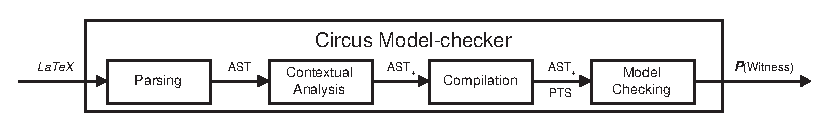
\epsfig{clip=, scale=0.9,
    file=mc.arch.stages.eps} \end{center} \caption{\Circus\ Model
    Checking Stages}\label{mc-stages} \end{figure} The theorem
    proving module presents both in the compiler and refinement engine
    dispatches requests for evaluation of Z expressions and predicates.
    These are either verification conditions over the state operations
    defined in Z, or possible enabling paths available for investigation
    from the behavioural actions given using CSP.  At this point theorem
    proving is usually necessary to discharge proof obligations, and
    simplify expressions or predicates. Nevertheless, for
    specifications with simple state operations, animation is also a
    good idea that can improve the automation of the model checking
    process.

    The role ZLive plays in this architecture is to tackle the
    requests to evaluate Z expressions and predicates from the
    compiler and refinement engine.  As the operational semantics of
    \Circus\ is given in Z itself, we can use ZLive as a meta-level
    animator for simple specifications, hence enabling automatic model
    checking of state-rich \Circus\ specifications.  With few
    improvements and extensions to the current implementation of ZLive
    to handle more of the schema calculus, we expect this to be a good
    example of how to integrate different CZT tools across different
    paradigms and tool boundaries. Furthermore, as the theorem proving
    integration architecture of the \Circus\ model checker allows
    pluggable solutions suitable for individual contexts, if ZLive
    cannot handle some complex \Circus\ specifications, we can still
    resort to some alternative solution such as SAT solvers, and
    general-purpose theorem provers.

\section{Specification Manager}
\label{section-manager}

  One of the core components of the CZT framework is the
  \emph{specification manager}, which is an extensible repository for
  formal methods objects.  Most of the tools mentioned in the previous
  sections use the specification manager to enquire about specific
  aspects of a specification.  For example, to be able to parse a Z
  section, the Z parser needs the operator definitions of the parent
  sections.  In order to typecheck a Z section, the section must be
  parsed and the parents of that section typechecked.  To print a Z
  section in \LaTeX\ markup, the operator definitions and \LaTeX\
  markup directives of the parent sections are needed.

  While it would be possible to hard-code these dependencies and let,
  for example, the \LaTeX\ markup printer call the parser for the
  parent sections directly, it is more convenient, extensible, and
  efficient to have a central repository that is responsible for this
  task.  The CZT specification manager caches information about all
  the specifications and Z sections that are being processed and
  automatically runs tools such as markup converters, parsers and
  typecheckers when necessary.  The caching of the parsed form of
  commonly used objects, such as standard toolkit sections, avoids
  repeated parsing and analysis of these objects and can give
  significant performance improvements.  Abstractly, the cache is a
  mapping from a key to the actual data.  The key is a
  $(String,Class)$ pair, where the $String$ is usually the name of the
  section, and the $Class$ is the Java class of the type of data
  associated with this key.  This allows several different kinds of
  objects to be associated with one section, and provides some dynamic
  type security.  For example, the Z parser adds the AST of a
  specification it has parsed to the specification manager.  The type
  of a Z section in Java is \Interface{ZSect.class}. Thus the AST for
  a section called \texttt{foo} is cached under the key
  \texttt{(``foo'',~ZSect.class)}.

  The CZT specification manager supports two important kinds of
  extensibility:
  \begin{description}
  \item[Type Extensibility:] Z extensions can easily use the
    specification manager to store new types of information, since the
    flexible $(String,Class)$ key system allows arbitrary Java objects
    to be stored and retrieved.  That is, the kinds of objects managed
    by the specification manager are open-ended, rather than being a
    fixed set of Z-related objects.
  \item[Command Extensibility:] A Z extension can easily add or
    override the \emph{default commands} of the specification manager.
    The default commands of the specification manager are responsible
    for automatically computing requested objects;~they are
    implemented using the command design pattern~\cite{GamEA:95}. For
    example, if the AST (i.e. data of type \Interface{ZSect.class})
    for section \texttt{foo} is required and has not already been
    cached, the Z parser is called by the specification manager in
    order to parse the specification file containing section
    \texttt{foo}.  Here, the Z parser is the default command to
    compute data of type \Interface{ZSect.class}.  A Z extension that
    needs to use a different parser can simply override the default
    command associated with the type \Interface{ZSect.class}.  For
    example, the specification manager can be configured to always use
    the Object-Z parser.
    \end{description}

  A major advantage of this default command approach is that it
  simplifies tool development and makes tools more flexible, because a
  particular tool does not have to know which other tools to use in
  order to find information about a section --- it simply requests the
  key that it wants and the specification manager will locate the
  information if it is able.  This gives a more flexible,
  \emph{plugin} style of tool development.

\section{Conclusions and Future Work} \label{sec:conclusions}

\bibliographystyle{splncs}
\bibliography{ifm}

\end{document}
